% ------- Create Preamble ------------
\documentclass [12pt]{article} 
\usepackage[a4paper]{geometry} 
\usepackage{amsmath, amsthm, amssymb, amsfonts}
\usepackage{graphicx,epsfig}
\usepackage{booktabs} 
\usepackage{pslatex} 
\usepackage{caption} 
\usepackage{setspace} 
\usepackage{hyperref} 
\usepackage{multicol, multirow}
\usepackage{graphicx,epsfig}
\usepackage{booktabs}
\usepackage{pslatex}
\usepackage{caption}
\usepackage{setspace}
\usepackage{hyperref}
\usepackage{multicol}
\usepackage{textgreek}
\usepackage{pdfpages}
\usepackage{longtable}
\usepackage{float}
\usepackage{natbib} % For references
\bibpunct{(}{)}{;}{a}{}{,} % Reference punctuation
\def\citeapos#1{\citeauthor{#1}'s (\citeyear{#1})}
\newtheorem{hypothesis}{Hypothesis}
\newtheorem{nullhypothesis}{Null Hypothesis}
\usepackage{xcolor}
\hypersetup{
	colorlinks,
	linkcolor={blue!50!blue},
	citecolor={blue!80!blue},
	urlcolor={blue!80!blue}
}

\usepackage{indentfirst}

\usepackage{booktabs}
\usepackage{siunitx}
\newcolumntype{d}{S[input-symbols = ()]}


\widowpenalty=5000
\clubpenalty=5000

\usepackage{fancyhdr}
\pagestyle{fancy}
\fancyhf{}
\rhead{Garrett and Roberts}
\lhead{\textit{Don't Interrupt Me}}
\rfoot{Page \thepage}

%---Set up author and title page
\singlespace
\title{Don't Interrupt Me: The Interruption of Female and Nominees of Color in Federal Judiciary Confirmation Hearings}
\author{Tyler Garrett\footnote{Ph.D. Student, Department of Political Science, University of Colorado Boulder, UCB 333, Boulder, CO 80309-0333. Tyler.Garrett@colorado.edu} \and Damon C.\ Roberts\footnote{PhD Candidate,
		Department of Political Science, University of Colorado Boulder, UCB 333, Boulder, CO 80309-0333. Damon.Roberts-1@colorado.edu. \newline \textbf{Note: Author name order is alphabetical.} \newline \textbf{Acknowledgements:} We'd like to thank the American Political Research Lab at the University of Colorado Boulder for their advice and we'd like to thank Alexdandra Siegel for her advice and for her support. \newline \textbf{Project Code:} \href{https://github.com/DamonCharlesRoberts/judiciary_hearing_interruptions}{Found on Github - https:://github.com/DamonCharlesRoberts}}}

%set up document
\date{Updated: \today}

\begin{document}
	\maketitle
	\begin{abstract}
A common expectation is that the nomination process of federal court judges have become relatively more conflictual as polarization in Congress has increased over time. We expect that the degree to which one is treated differently by members of the committee is not just the result of partisanship but also based on one's ascriptive characteristics like gender and race. By quantifying text, we examine female nominees and nominees of color face biases irregardless of their political leanings. Through the analysis of transcripts from the Senate Committee for the Judiciary from 2001-2020, we found some evidence that warrants further investigation that female nominees and nominees of color are treated differently during their confirmation proceedings. While we find no support for differences in the number of interruptions of nominees, female nominees and nominees of color do encounter differences in the conversations they have relative to their white male counterparts.
	\end{abstract}
	
	\textbf{Word Count: ??} 
	
	\textbf{Keywords: Gender, Race, Judicial Politics, Text Analysis, Transcripts}

	\cleardoublepage
    \setcounter{page}{2}
	\newpage
	\doublespace
	\newpage 

\section{Introduction}
	
Many streams of the literature in political science are concerned with the ways in which particular institutional and societal biases affect the degree to which one is able to exert voice in political settings. In Congress, for example, women are often presumed to be more collegial and more adept at arranging events for the branch \citep{lawless_2018}, women are less likely to have the opportunity to express an opinion in many common settings with political deliberation  \citep{karpowitz_et-al_2012}, and female Justices on the Supreme Court are more likely to be interrupted by their male colleagues than they are to interrupt them \citep{jacobi_2017}. It is not only along the dimension of gender that we see these biases occur, however. When intersectional identities are at play, the voices of members of these groups are often drowned out by those of males and whites \citep[see][for example]{strolovitch_2006}. We are likely to see these effects happen, in particular, for nominees of various positions with the federal court system. 

Furthermore, examples of either gendered or racialized questions and comments by senators during the confirmation processes are prevalent even today. During the confirmation of Amy Coney Barrett to the United States Supreme Court—the highest court in the land—Senator John Kennedy of Louisiana asked the nominee about who does the laundry at her home. It does not appear that Senator Kennedy asked other recent Supreme Court nominees Neil Gorsuch or Brett Kavanaugh—both white men—who does laundry in their house. This same questioning did not occur with any other nominee. With the announcement from the Biden administration that they were nominating Ketanji Brown Jackson to the Supreme Court to replace Breyer, Tucker Carlson appeared on his program aired by Fox News to question Jackson's qualifications by demanding to see her LSAT scores, racistly implying her success has come from affirmative action.  In light of a number of highly polarizing and recent confirmation hearings for nominees to federal judicial positions - Justices Gorsuch, Kavanaugh, and Coney-Barrett, in particular - this manuscript seeks to determine whether these common gender and racial biases documented in previous work present themselves in the transcripts of confirmation hearings for federal court positions. 

In this study, we set out to determine if female and nominees of color are treated differently than their white and male counterparts during their confirmation proceedings before the Senate Judiciary Committee. If they are treated differently, then this contributes to the barriers that female and nominees of color face when navigating yet another hurdle in the advancement of their legal careers. Further, support of this hypothesis would pose a direct challenge to claims that the lack of non-white and female representation in the federal court system is the result of supply from law school or qualifications. While finding evidence of our hypothesis would not necessarily show that nominees of color and female nominees are held to a \textit{higher} standard - as we do not test this, evidence in support of our hypothesis would demonstrate that they are held to \textit{different} standards.

In two studies we explore whether female and nominees of color were treated differently than their white and male colleagues. First, we tested whether female and nominees of color are interrupted at a higher rate than their white and male colleagues. We find mixed results. In the second study we set out to determine if the topics during confirmation hearings for female and nominees of color bring up different topics than those discussed during confirmation hearings for white and male nominees. Our analysis found that there are some substantive differences in the topics that are discussed during the confirmation processes of female and nominees of color than their white and male counterparts. As in the example of Amy Coney Barrett above, the substantive differences in topics discussed in the confirmation processes of female and nominees of color consist of both racial and gendered stereotypes that are prevalent in politics and society today. 

We start our study with a discussion of the motivating literature around this topic of how women and people of color as either nominees or as actors within the federal government have been treated differently. Particularly, we will focus on how these individuals are treated during in a group dynamic amongst other governmental actors. We will then briefly discuss our theory and how we plan to build upon those who have come before us in this important literature. Following our discussion of our theory, we will lay out how we conducted our study—from the collection of transcripts for Senate Judiciary Committee hearings on confirmations for federal judges and justices, sorting the data, determined interruptions and then set out at analyzing the data on the discrepancies between white male nominees and nominees of color and female nominees. Following our analysis and discussion of results, we will conclude with the impact of this study, a discussion of future iterations of this project moving forward, and discussing avenues for future research related to this study. 

	\subsection{Political biases around race}
On the dimension of race, there have been only 2 Black justices and one Hispanic justice. We have yet to see an Asian-American justice, indigenous justice, or justice of any other race or ethnicity. Since the Carter Administration, presidents have paid closer attention to the gender and racial diversity of their nominees \citep{kastellec_2013}. 

\section{Biases in politics and the courts}

Stereotypes based on gender in politics are quite common and are quite well documented. Women are assumed to be more liberal \citep{mcdermott_1997_ajps}, more warm due to gender stereotypes and their connection to sex \citep{laustsen_bor_2017}, and are assumed to be less competent at addressing salient policy issues like crime \citep{huddy_terkildsen_1993, sanbonmatsu_dolan_2009}; which are assumed to be more masculine \citep{holman_et-al_2016}. With all of these electoral biases, women are less likely to be considered for higher public office \citep{oliver_conroy_2020} and if they attain office, are more likely to face stronger criticism for the work they do \citep{lazarus_steigerwalt_2018}.

Stereotypes based on race are also widespread and pervasive. Holding negative racial attitudes is attributed to not just be among the predictors of vote choice and policy support \citep{sides_et-al_2018, gilens_1999}, but it is argued to be \textit{the} predictor of such evaluations; more so than class \citep{hajnal_2020}. If you take the average white respondent who are unsupportive of welfare programs, which the media frames as disproportionately beneficial to Black Americans, they argue it is not that they dislike the programs themselves but that they feel that Black Americans are ``undeserving" \citep{winter_2008}. Though many view these attitudes as driven by older voters when comparing cohorts on the Kinder and Sanders \citeyearpar{kinder_sanders_1996} racial resentment battery, a more generation appropriate battery demonstrates that millennials are just as racially conservative as previous generations \citep{desante_smith_2020_chicago}. Additionally, non-white candidates, specifically African American candidates like Obama, feel pressure by White segments of their electorate to ``distance" themselves from their African American voters due to the tendency for White voters to dislike candidates ``beholden" to a particular racial group's interest \citep{stephens-dougan_2020}; except for their own that is. In some ways the courts are reflections of these same emergence and continuing biases that women and people of color face while running for political offices. As there is little reason to believe that these biases somehow stop at the courthouse footsteps, we believe that some of these phenomenon may also be present in some form in the federal courts.

The majority of judges and justices on the federal courts in the United States are white men \citep{kastellec_2013}. Since the Court was established in 1789, there have been only 5 female justices out of the 115 justices to serve on the United States Supreme Court. Although there have been a growing number of female and nominees of color to the federal judiciary, the path to the bench upon being nominated is not always easy. The confirmation processes for female nominees and nominees of color are longer with a lower outcome of success \citep{asmussen_2011}. Part of this is likely due to the increase in polarization in Congress--particularly in the Senate Judiciary Committee--since the Carter Administration, which has catastrophic effects on the norms of the Senate \citep{owens_2018, mccarty_et-al_2005}. It is evident in the literature that the role of partisan politics in confirmation processes for female and nominees of color has created even more arduous proceedings than previously \citep{solowiej_2005}. 

Not only are female nominees and nominees of color facing the possibility of longer confirmation hearings with less confidence of success \citep{asmussen_2011}, the nominees also face questions that their white and male colleagues do not--this is common for female and nominees of color for the federal judiciary and for elected positions \citep{boyd_2018, hayes_2015, devitt_2002, palmer_2010, schultz_1997}. Whereas male candidates for office will often get questions about the issues, female candidates are faced with those questions and questions about their personality and qualifications \citep{devitt_2002}. We expect this to hold as true in the context of confirmation hearings to the federal bench as it does for political candidates. Finally, female nominees for the Supreme Court (as well as for Cabinet positions) are faced with a higher rate of questions pertaining to their qualifications, personality, stance on ``women's issues" and their appearance than their male colleagues \citep{boyd_2018, hayes_2015, devitt_2002, palmer_2010, schultz_1997}. Once they have joined the court, scholars have documented a continuation of these gender and race-based biases.

While a constant barrage of questions from the justices on the Supreme Court is normal, there has been a trend emerging that breaks with the norms of the Court. While it was normal for the justices to occasionally interrupt each other, we have seen an increase in the justices speaking over one another to ensure that their question is answered \citep{jacobi_2017}. The interruptions are not equal though amongst the justices. Female justices are interrupted at a higher rate by their colleagues than male justices \citep{jacobi_2017}. Furthermore, female justices are interrupted more by attorneys at higher rates than their male colleagues \citep{jacobi_2017}. This is astounding and unprecedented. Although the attorneys arguing before the Supreme Court are at the top of their field and most likely experts in the area of law present in the case, interrupting a Supreme Court justice while they are sitting on the bench is a major faux pas. The justices are typically treated with an incredible amount of respect, yet interrupting a justice seems to indicate a diminishing lack of respect. 

The study by Jacobi and Schweers \citeyearpar{jacobi_2017} was a major motivation for our study. We were perplexed by the audacity of attorneys to interrupt sitting Supreme Court justices and the indication of inherent sexist tendencies that the female justices must contend. We figure that if the individuals that sit on the highest court of the land can face such actions while on the bench, they and their colleagues that are nominees for lower level courts must face similar situations during their confirmation hearings before the Senate Committee on the Judiciary. Particularly, when there is this veil shielding those expressing the biases as the result of ``ideological disagreements."

Building on this literature, we set out to determine in a descriptive study if female nominees and nominees of color are treated differently than their white and male colleagues. Given the literature above, we highlight two hypotheses meant to describe descriptive patterns.

\begin{itemize}
\item[\textit{$H_1$}:] There are gendered-and-racially-based differences in how federal judicial nominees will be treated during their confirmation hearing before the Senate Committee on the Judiciary.
\begin{itemize}
    \item[\textit{$H_{1a}$}:] Female nominees for federal judicial appointments will be interrupted at a higher rate during their confirmation proceedings than their white male colleagues. 
    \item[\textit{$H_{1b}$}:] Nominees of color for federal judicial appointments will be interrupted at a higher rate during their confirmation than their white male colleagues.
\end{itemize}

\item[\textit{$H_2$}:] The Senate Committee on the Judiciary will discuss topics with gendered or racialized connotations if there are female and nominees of color as opposed to their white male colleagues. 
\begin{itemize}
    \item[\textit{$H_{2a}$}:] Female nominees will face a higher rate of questions and focus on topics associated with gender than male nominees. While there are a number of such topics, we might expect more focus on topics around the female nominee's family as this is a common trope of career-oriented women and is a common challenge to female candidates for political office \citep[see][]{sanbonmatsu_dolan_2009}.
    \item[\textit{$H_{2b}$}:] Nominees of color will face a higher rate of questions and focus on topics associated with their qualifications and their views on equity than white nominees. Again, there are a number of topics that may be ``racialized", however, previous literature shows that, on the whole, the electorate - particularly the white electorate - are much less supportive of non-white candidates who do not actively distance themselves from those in their community \citep{stephens-dougan_2020}. We also know that it is common for Americans to bring about questions of deservingness for people of color in the U.S.\citep{gilens_1999};much of it stemming from resentment towards affirmative action.
\end{itemize}
\end{itemize}	

In order to determine if there are any differences in the way that female and nominees of color are treated compared to white and male nominees, we focus on interruptions. As we have seen, female justices on the Supreme Court are being interrupted at a higher rate than male justices and lawyers will even interrupt the female justices \citep{jacobi_2017}. This leads us to expect that there would also be a difference in the way that female and nominees of color would be treated by senators during their confirmation proceedings. We expect before running the analysis that female and nominees of color would be interrupted by the senators at a higher rate than white and male nominees. Additionally, female nominees of color would be interrupted at the highest rate. If interruptions were higher for female and nominees of color, then we would be able to say that there are gendered and racially motivated norms for how female and nominees of color are treated during their confirmation hearing. We, ultimately, find mixed results, which lead us to consider that instead of the sheer volume of interruptions we need to determine the motivation behind the interruption.

As for the second hypothesis, we again need to determine if there is a difference in how female and nominees of color are treated during their confirmation hearings. Instead of interruptions though, we use topic models to determine if senators ask female and nominees of color more gendered and racialized questions than their white male colleagues. Other than blatant gendered and racialized questions, a higher number of questions about the nominees intellect, commitment, qualifications, and experience would also lead us to believe that the committee is adhering to unfair norms that emulates themselves in the form of gendered and racialized questions and comments for the nominees. We do find that there are some differences between the topics discussed during the confirmation hearing between male and female nominees and white nominees and nominees of color.

\section{Methods}

We conduct two studies. The first study is concerned with testing our first set of hypotheses that predict differences in the number of interruptions a nominee experiences due to their gender and their racial status. The second study then is tasked with determining whether there are differences in the topics that are discussed during a nominee's committee. As noted above, while it is possible that nominees experience more or less interruptions based on their demographic characteristics, those biases are likely not limited to only that - the topics of which are brought up to determine one's qualification for the role is likely to be different based on commonly held racial and gender biases. Study 2 uses the same transcript above, but uses topic models to study these hypothesized dynamics.
	     
For both studies we collected data from the Senate Judiciary Committee's website where they publish PDF documents of transcripts from their committee hearings. We found the documents containing the transcripts from the confirmation hearings for federal appointments held from 2001 until 2020. We chose this time period to capture hearings from a reasonable time period where we have a sample of nominees presented by both Republican and Democratic presidents. We wanted to also ensure that since the hearings of a few of President Donald J. Trump's nominees were quite publicly polarizing, that we had nominees from a Republican president like George W. Bush who's nominees were somewhat less controversial. Once we had collected these documents, we used data from the Federal Judicial Center \footnote{\href{https://www.fjc.gov/}{Federal Judicial Center}} which we used to leverage demographic information about the federal nominees to assign each of the transcripts to labels based on whether the nominee was a Male or Female and whether they were a Person of Color (POC) or not. Once we completed this manual coding we preformed a Regular Expression content matching to separate the lines of the transcripts where people spoke. Line breaks were consistently recorded throughout the transcripts as ``\textbackslash n \textbackslash r" while new lines started with the title capitalized along with the last name of the speaker followed by a period (e.g. SENATOR MERKLEY.) Additionally, we used the list of nominees contained in the Federal Judicial Center data of judicial nominees to select the lines where a nominee spoke and filtered out the comments made by the committee members. Once we had this filtered text, we again used Regular Expression matching to get an aggregated count over the course of a hearing for the number of times a candidate was interrupted; thankfully, interruptions were consistently recorded in the transcripts as em-dashes followed by a line break (i.e. ``\textbackslash r \textbackslash n"). 
	
The count of interruptions recorded for a particular nominee in their hearings are presented in Figure \ref{fig:1}. We excluded the cases of Kavanaugh and Gorsuch in the figure due to the abnormally high count of interruptions they experienced in the hearing which were 556 and 386 respectively. The dashed line depicts the median count of interruptions which is 0, along with a dotted line depicting the location of the median which is 3.64.
	
	\begin{figure}[H]
	    \centering
	    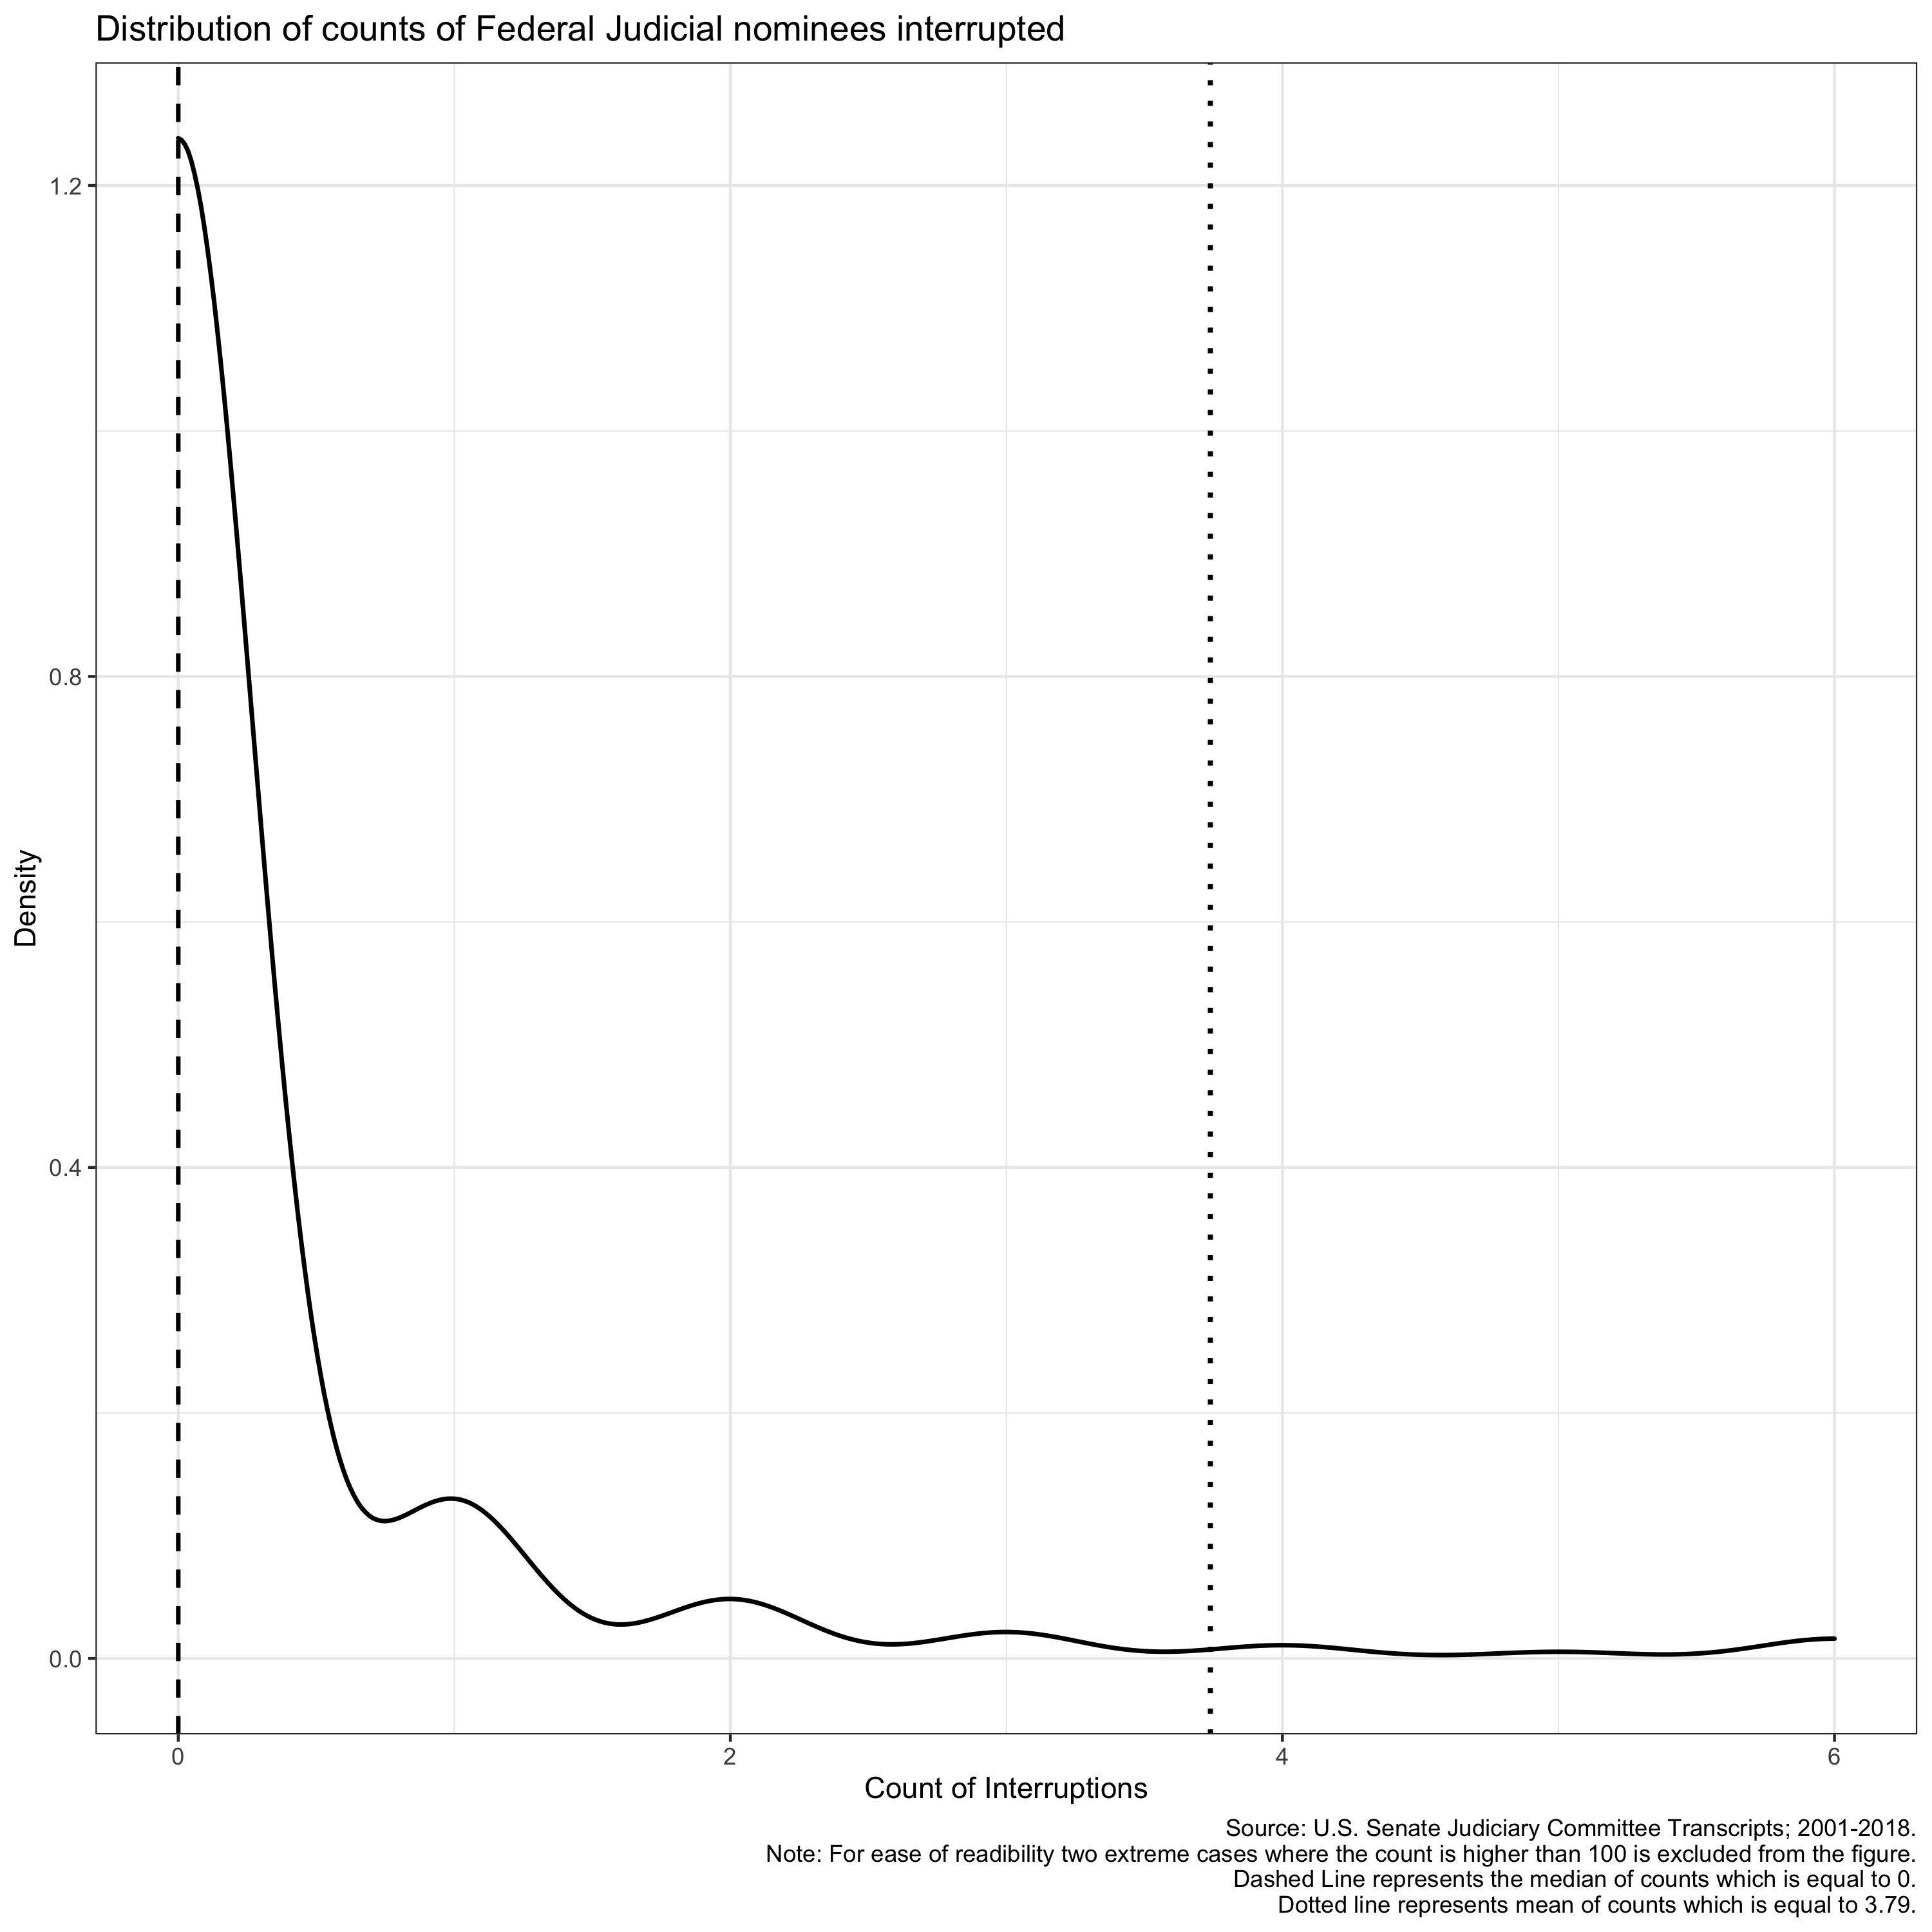
\includegraphics[height = 175mm, width = 175mm]{../tables_figures/interruptions_distribution.png}
	    \caption{Density of interruption counts}
	    \label{fig:1}
	\end{figure}
    
    We also present Figure \ref{fig:2} which is meant to demonstrate the descriptive differences in interruptions between male and female, and POC and non-POC nominees. Here, we see that most nominees do not experience too many interruptions over the course of their hearings.
    
    \begin{figure}[H]
        \centering
        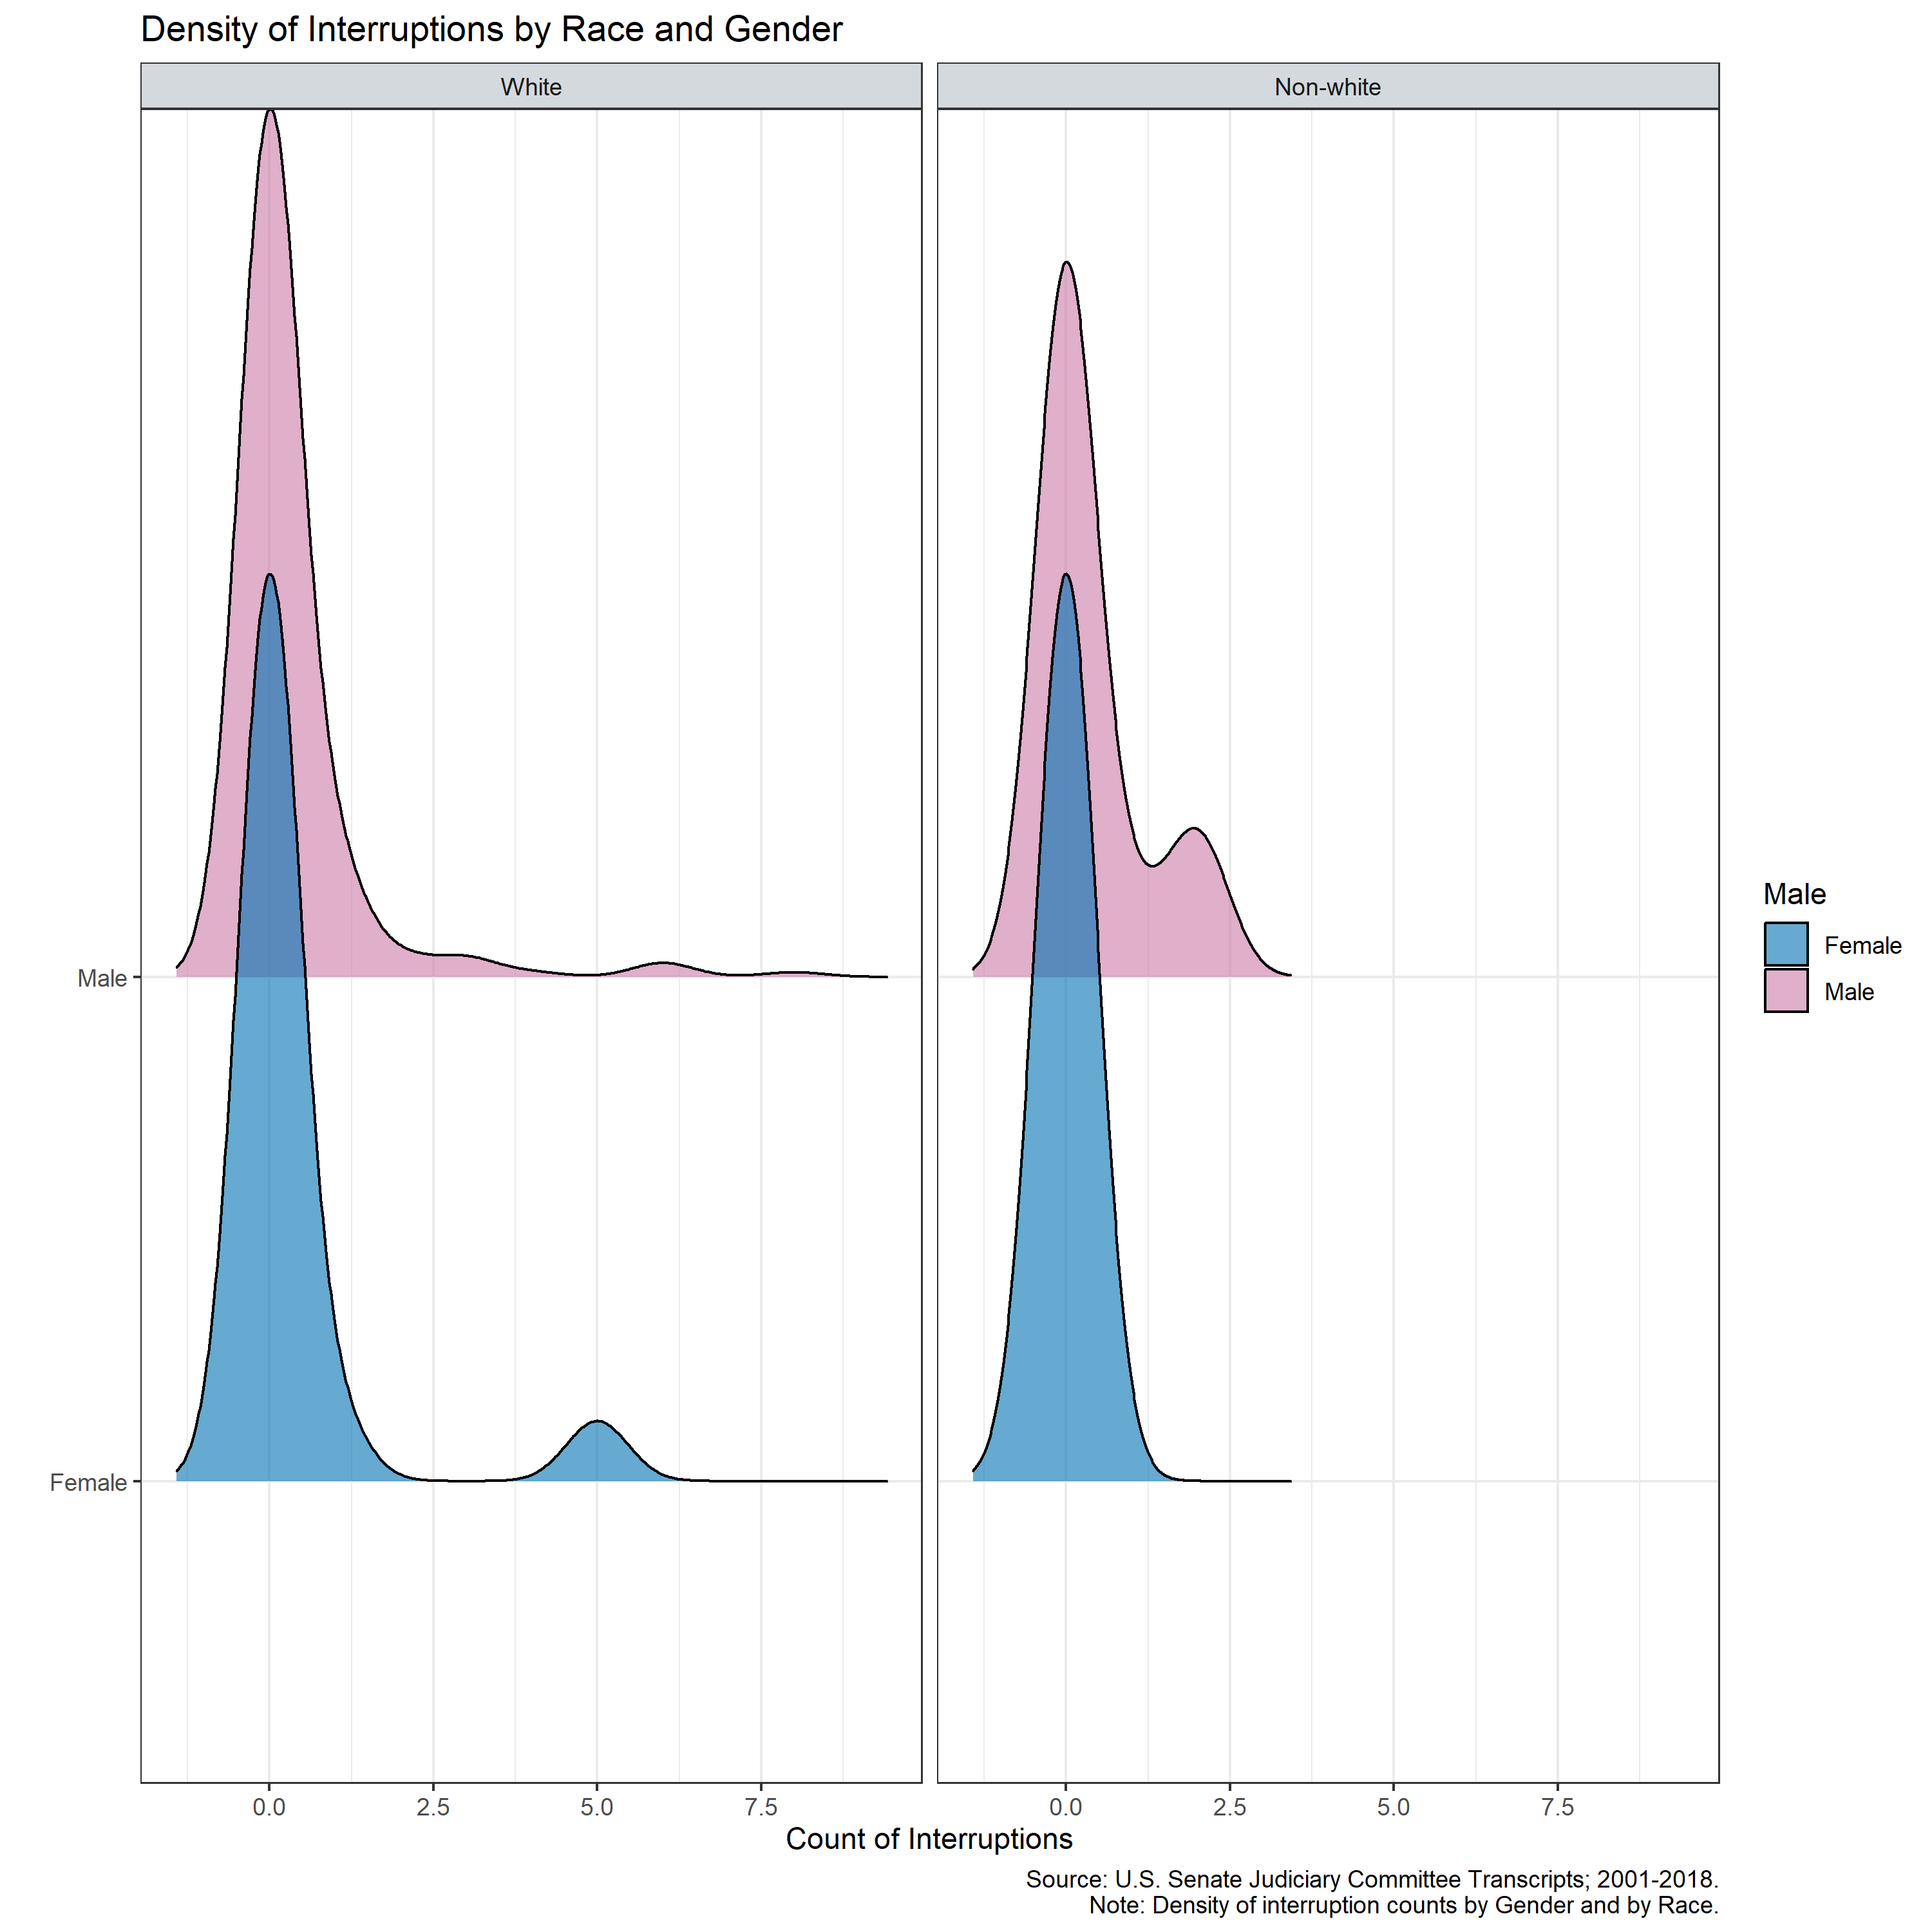
\includegraphics[height = 175mm, width = 175mm]{../tables_figures/interruptions_ridgeplot.png}
        \caption{Densities of interruption counts by Gender and Race}
        \label{fig:2}
    \end{figure}
    

    
\subsection{Study 1}
	    
The goal of our task here is not to make causal claims. We simply want to test the claim whether the number of interruptions a nominee faces are based on their gender or on their race. Keeping this goal in mind, we first use a simple unpaired two-samples Wilcoxon test \footnote{Rather than using a simple t-test, we use a non-parametric form which relaxes the distributional assumptions that are involved with standard student t-tests and $\chi$ tests. We include a figure for the results of the t-test as well in the main body of the text. The non-parametric Wilcoxon test is used over the t-test due to the variation between the distributions of counts on our sub-samples on race and gender. Since parametric tests often assume the comparability in distributions of our variables, as Figure \ref{fig:2} demonstrates, it seems somewhat inappropriate to use a parametric version of the test.} to determine whether there are descriptive differences for these considerations among the dichotomized social classifications. We also hypothesized that partisan disagreement over the nominee by the nominating president and the committee could be an important alternative explanation for the number of interruptions a nominee faces. Therefore we include a proxy for how favorable the committee is likely to be toward the nominee. We first collected information about the Senate Committee on the Judiciary's membership from the $107^{th}$ Congress until the $116^{th}$. Committee compositions that had a Republican majority were given positive values and if it was a Democratic majority, it was assigned negative values (the integer assigned was based on how many members more than the minority party). We then used these data to calculate whether there was a split between the party of the President that made the nomination and the partisan composition of the committee. If there was a division, the index was coded as 1 and 0 if there was no division. These alternative explanations tested in conjunction with our gender and POC variables in a regression analysis presented later.
	    
For our Wilcoxon Test we are comparing the means within nominee characteristics. That is, we split our sample to be based on whether the nominee was POC or they were not. We then took the counts of the nominees in the split sample and compared the counts between POC and non-POC nominees to see whether there were any substantive differences. We made this comparison for the other two characteristics (gender and partisan division) as well. We also ran Wilcoxon tests with the full sample and a sample where we exclude the cases of Gorsuch and Kavanaugh. The results of the Wilcoxon Test are presented in Figure \ref{fig:wilcox}. In terms of hypothesis testing, the dots depict the p-values of the variables. Any dot below 0.05 (first dashed line on the x-axis) or above 0.95 (second dashed line on the x-axis) would be considered support for the alternative hypothesis that there is a meaningful difference greater than zero. In terms of hypothesis testing, support for a null hypothesis (that we do not observe meaningful differences in the mean counts between the categories) would present itself as an overlapping between our dot (or the t-statistic) and the bar (the 95\% confidence interval). 
	   	    \begin{figure}[H]
	        \centering
	        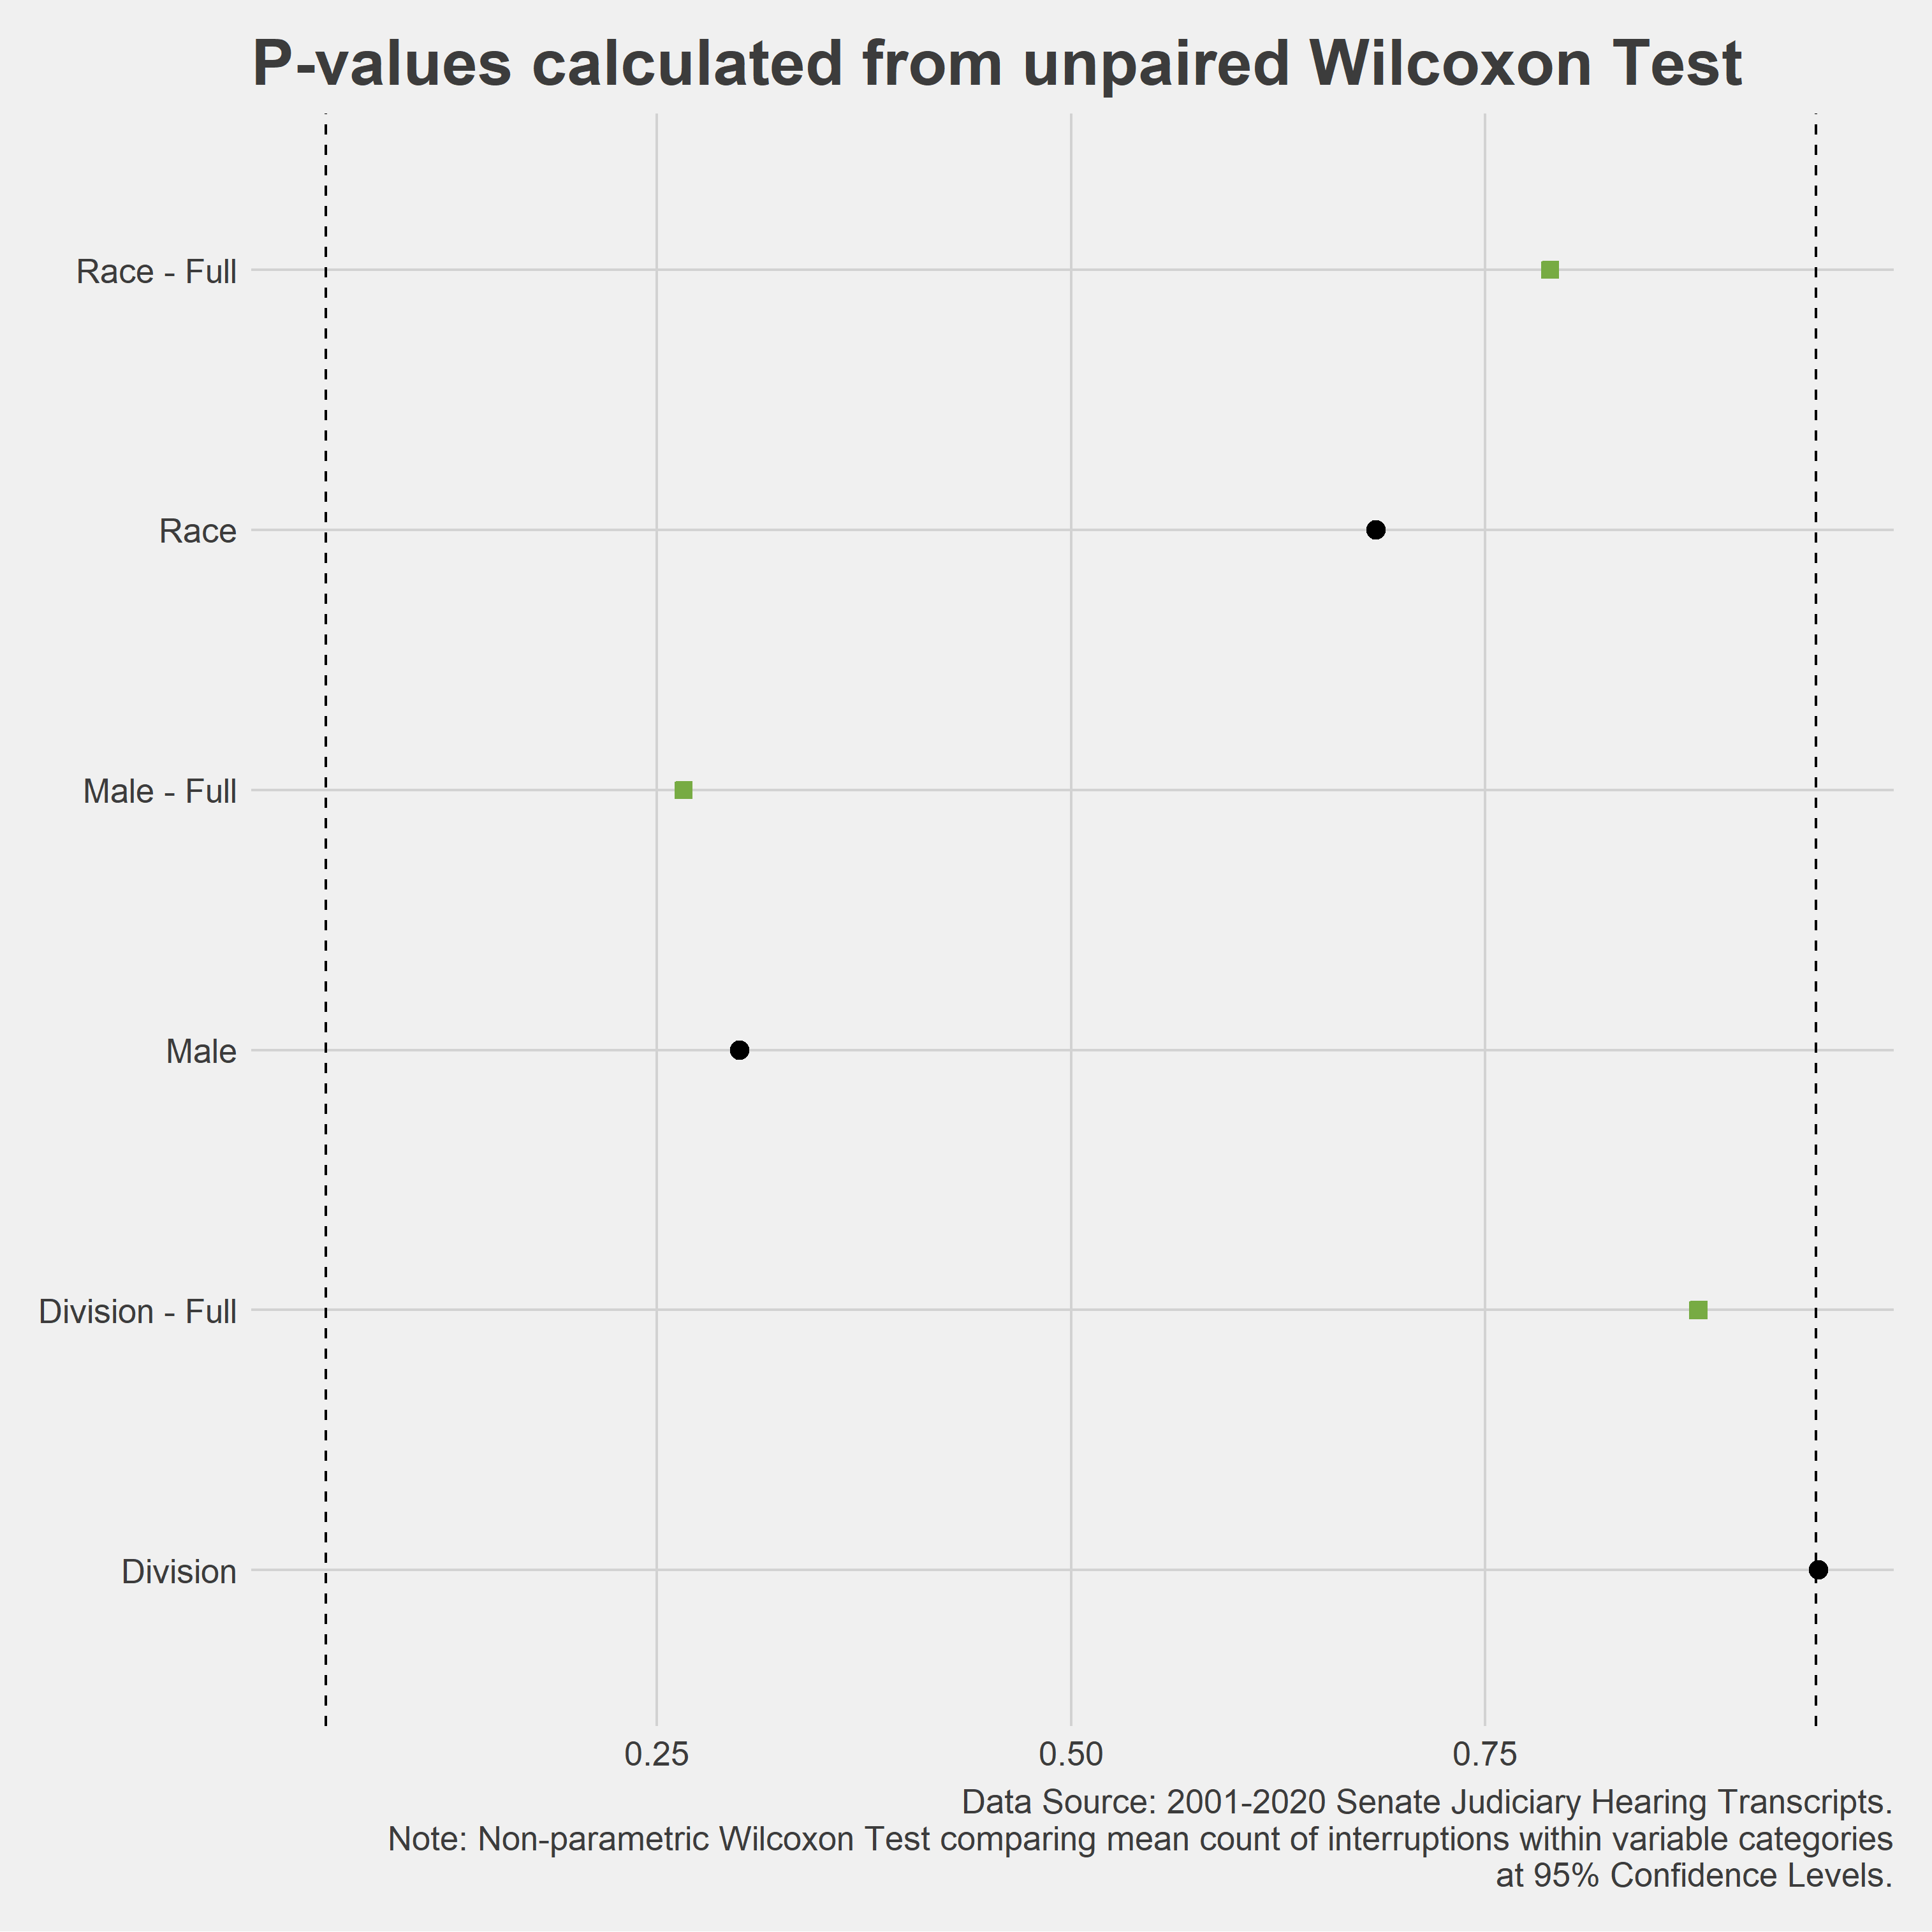
\includegraphics[height = 175mm, width = 175mm]{../tables_figures/wilcox-test.png}
	        \caption{Unpaired Two-samples Wilcoxon Test}
	        \label{fig:wilcox}
	    \end{figure}
	    

From the Wilcoxon test we observe that for both the full and the truncated dataset, our hypotheses on gender and race are not supported. The tests suggest that the mean counts of interruptions between Male and Female nominees and POC and non-POC nominees are not significantly different. We find support, however, for the hypothesis that there are meaningful differences between the mean counts of interruption between those nominated by a present of the opposing party than the majority party in the committee. This is only found in our censored dataset that excludes the cases of Gorsuch and Kavanaugh. From it we find that there is a positive relationship between division in government and the number of interruptions a nominee experiences. We are also interested in determining whether these characteristics matter in predicting the number of interruptions in multivariate setting. We expect that these factors all work together in some combination to influence the degree to which a nominee is interrupted. 

From Figure \ref{fig:2} we notice that there is a difference between the conditional mean and conditional variance of our interruption variable. It is not obvious that there is a separate data generating process leading to the high number of zeros, but we are not entirely sure. Given the difference between the mean and the median, we expect that a poisson distribution is not appropriate and so we use a poisson-gamma distribution in our estimation using the Negative Binomial Regression procedure.

We expect that along with the gender and the race of the nominee, their qualifications might influence the degree to which a nominee is interrupted. Those who are deemed less qualified by their peers (the American Bar Association) are likely to be interrupted more by members of the committee. Due to this suspicion, we include this variable as a control. Although we have clear expectations about the role that race, gender, and the partisan contexts in which a nominee may find themselves in will influence whether the nominee is interrupted, our expectations about their qualifications are not necessarily an alternative explanation for interruptions but is rather something that will likely have some influence on how many times a nominee is interrupted over the course of their confirmation hearing.	    
	    

% Table created by stargazer v.5.2.2 by Marek Hlavac, Harvard University. E-mail: hlavac at fas.harvard.edu
% Date and time: Thu, Apr 08, 2021 - 9:27:46 AM
\begin{table}[!htbp] \centering 
  \caption{Female and Nominees of Color interrupted more in confirmation hearings} 
  \label{} 
\begin{tabular}{@{\extracolsep{5pt}}lcc} 
\\[-1.8ex]\hline \\[-1.8ex] 
\\[-1.8ex] & \multicolumn{2}{c}{Count of Interruptions} \\ 
 & Full Cases & Excluded Extreme Cases \\ 
\hline \\[-1.8ex] 
 Person of Color & $-$0.635 & 0.083 \\ 
  & (0.932) & (0.571) \\ 
  Male & 2.086 & 0.107 \\ 
  & (1.151) & (0.689) \\ 
  Hearing Year & $-$0.278$^{*}$ & 0.012 \\ 
  & (0.066) & (0.043) \\ 
  ABA Qualified & $-$0.369 & 0.316 \\ 
  & (0.570) & (0.399) \\ 
  Division & $-$3.192$^{*}$ & 0.775 \\ 
  & (0.705) & (0.440) \\ 
  Constant & 557.317$^{*}$ & $-$25.646 \\ 
  & (132.735) & (86.502) \\ 
 N & 276 & 274 \\ 
Log Likelihood & $-$229.482 & $-$181.233 \\ 
$\theta$ & 0.053$^{*}$  (0.009) & 0.162$^{*}$  (0.041) \\ 
AIC & 470.964 & 374.466 \\ 
\hline \\[-1.8ex] 
\multicolumn{3}{l}{Source: 2001 - 2020 U.S. Senate Judiciary Hearing Transcripts.} \\ 
\multicolumn{3}{l}{Coefficients from Negative Binomial Regression Models.} \\ 
\multicolumn{3}{l}{Standard errors in parenthases} \\ 
\multicolumn{3}{l}{* p $<0.05$} \\ 
\end{tabular} 
\end{table} 


In our discussion of Figure \ref{fig:1} above, we noted that we excluded two points from the figure for readability - the hearing for Gorsuch and the hearing for Kavanaugh. Since both nominees were white males and were embroiled in highly salient and controversial hearings, we exclude their hearings from our analyses in the second column of Table \ref{tab:neg_binomial} in hopes of determining whether these are influential points biasing our results. We see that this is indeed the case. Our results appear quite different when excluding the cases of Gorsuch and Kavanaugh. We still do not find evidence for our hypotheses. It appears that the interruptions a nominee experiences might just be tied to whether or not there is controversy around their nomination. In terms of direction of the effect of division on interruptions, these conform with expectations about the hyperpolarization a number of scholars have observed in elite behavior when we include all cases \citep{mccarty_et-al_2005, ramey_2017, enders_2020}. Specifically, we find that more recent hearings have approximately 0.2 fewer interruptions than the previous year did on average. We also observe that when the committee is divided, there are about 3 fewer interruptions in a given hearing than when it is less divided. 
	    
\subsection{Discussion of Study 1}
	    
Comparing these results to those of the difference of means test, one might be alarmed by the difference in our results, we are not, however. The cases of Gorsuch and Kavanaugh were heavily partisan but were asymmetrically so. Both Gorsuch and Kavanaugh were nominated by a controversial Republican president and were controversial figures themselves. Therefore, this asymmetry is likely to make the split sample mean quite high. As a result we might expect that if there are equally controversial nominations by a Democratic president that record similar counts of interruptions, we should see that the differences between the full and the censored dataset would be closer to zero. Although the results of Study 1 do not support our hypothesis, as we allude to in our theory, we might expect that although there might not be more interruptions, there may be other forms of bias along the nominee's characteristics. Study 2 seeks to explore this speculation.
	    
\subsection{Study 2}
For Study 2, we implement a structural topic model, with the goal of determining whether the topics that are discussed in hearings are different between gender and racial categories. First, we take all text from the hearings and clean it in the same way that we did earlier (making a row per comment then aggregating them on speaker). This time, however, we do not exclude comments made by the committee members. We preform the standard pre-processing steps in text analysis by stemming words, removing punctuation, etcetera. 
	    
We run two models; one that we later use to regress the race of the nominee on what topics were discussed during their hearings as defined by the STM model and another on the gender of the nominee. We do this with the goal of being able to predict differences in what topics were discussed for the nominees based on their race and their gender. 

Topic models are useful for discovering patterns in text data that are much harder for humans to pick up on. These models do not reduce the burden of making explicit choices that affect the model's output \citep{grimmer_et-al_2022}, but there are a number of tools and metrics one can use to examine whether the model picked up on meaningful patterns and did so reliably. First, as we expect there to be a larger set of topics covered over the close to 20 years of transcript data, we use the \verb|searchK| function to help identify an optimal number of topics between 10 and 30. In doing so we also specify a Spectral Initialization as opposed to LDA's Gibbs Sampler to improve replicability \citep[see][]{roberts_et-al_2019}. As our theory expects that the prevalence of these topics depends on nominee race and gender, we use this function twice, once where the prevalence is determined by race and once where it is set to gender. We set the upperbound of 30 topics partly as a result of computational capability concerns\footnote{With a desktop that was only running the models through a bash terminal instance and a text editor, with 64 Gb of RAM, it still took more than 8 hours for the first set of the models to converge.} (it runs a structural topic model with 10 topics, then 11, then 12, then 13, etc. and stores this information), and out of concern for parsimony. To confirm that an upperbound of 30 topics, we also looked for an inflection point in the difference between topic model performance with metrics such as semantic coherence, residuals, held-out likelihood, and lowerbound. Details about what these metrics mean are discussed in a great description of the STM package by Roberts and colleagues \citep[see][]{roberts_et-al_2019}. To us, the inflection point comparing within these various metrics across models with a different number of topics represent a small gain in model performance but an increase in cost in terms of interpretability and in computational complexity. Figure \ref{fig:search_k_performance} present the performance of the models across number of topics for race, the top panel, and gender, the bottom panel. As we expected, looking at a specification of the models with 30 topics using a Spectral initialization and the prevalance of the topics determined by race and gender seems to perform much better across the metrics to a model with 20 or even 25 topics. 

\begin{figure}
	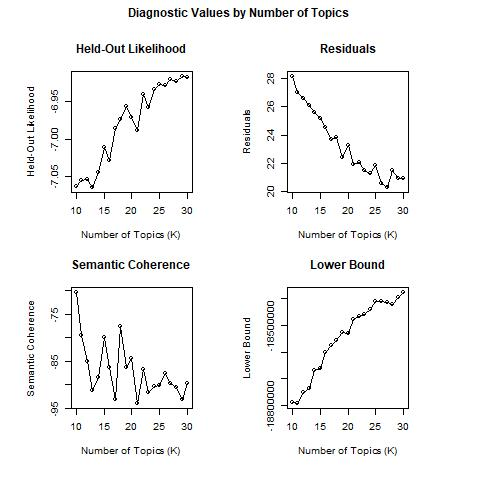
\includegraphics[width = 125mm]{../tables_figures/search_k_poc.jpeg}
	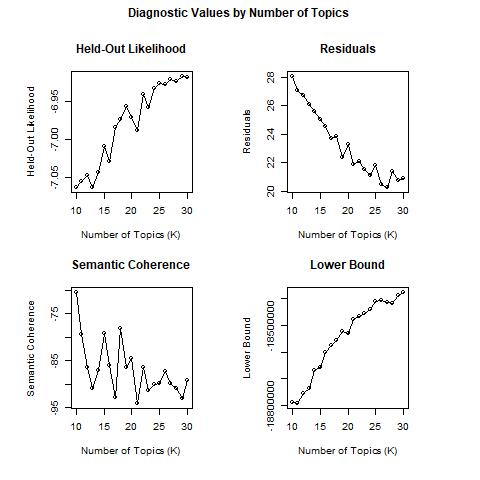
\includegraphics[width = 125mm]{../tables_figures/search_k_male.jpeg}
	\caption{Model metrics across number of topics}
	\label{fig:search_k_performance}
\end{figure}

Knowing that for both race and gender, 30 topics seems to be the most appropriate number of topics for our model, we rerun the model using the \verb|stm| function where we use the spectral initialization, specify that the prevalance of the topics are dependent on race and run the model again but with gender. With the models trained, we then seek to examine whether race and gender separately predict the topics. Therefore, we run two separate regressions. The result of these predictive regressions are presented in Figures \ref{fig:stm_poc} and \ref{fig:stm_male}. To note, in Figure \ref{fig:stm_poc} as you move up in values on the x-axis, it depicts the coefficient for nominees of color. Likewise in Figure \ref{fig:stm_male}, as you move up values on the x-axis, it depicts the coefficient for male nominees. 

\begin{figure}[H]
    \centering
    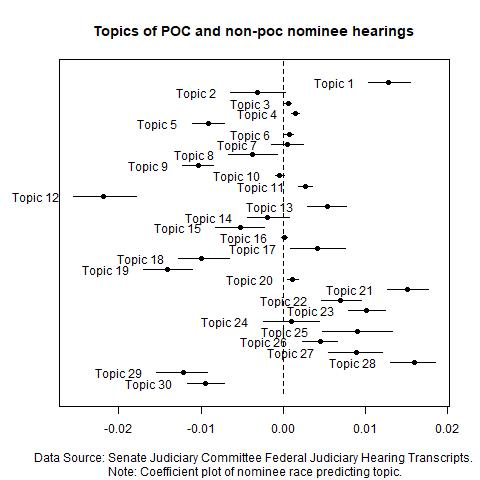
\includegraphics[height = 175mm, width = 175mm]{../tables_figures/stm_poc_predict.jpg}
    \caption{Predicting topic from nominee race}
    \label{fig:stm_poc}
\end{figure}
\begin{figure}[H]
    \centering
    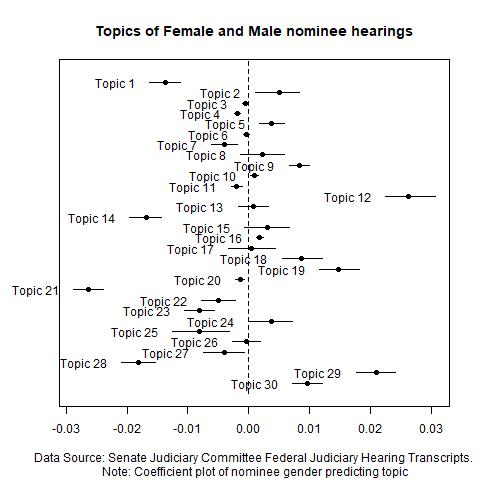
\includegraphics[height = 175mm, width = 175mm]{../tables_figures/stm_male_predict.jpg}
    \caption{Predicting topic from nominee gender}
    \label{fig:stm_male}
\end{figure}

\subsection{Discussion of Study 2}

We see that there are a number of topics that are different depending on whether you are a nominee of color or female. In Figure \ref{fig:stm_poc}, we see that topics 1, 23, 25, and 28 have a positive correlation with nominees of color and topics 5, 8, 12, 17, 19, 29, and 30 are noticeably associated with white nominees. In Figure \ref{fig:stm_male} most notably associated with male nominees are topic 9, 12, 18, 19, 29, and 30; topics 1, 7, 14, 22, 23, 25, and 28 are most notably positively associated with female nominees. So there are difference in the topics that are brought up during the confirmation hearings for both nominees of color and female nominees from their white male counterparts.

\begin{figure}[H]
    \centering
    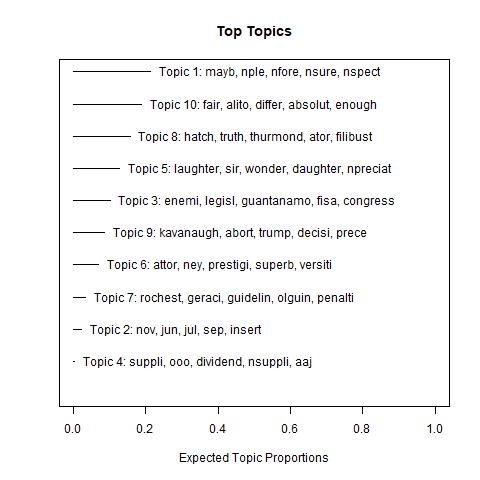
\includegraphics[height = 175mm, width = 175mm]{../tables_figures/stm_poc_frex.jpg}
    \caption{Predicted proportion of topics with 5 top words based on their FREX.}
    \label{fig:frex_poc}
\end{figure}
\begin{figure}[H]
    \centering
    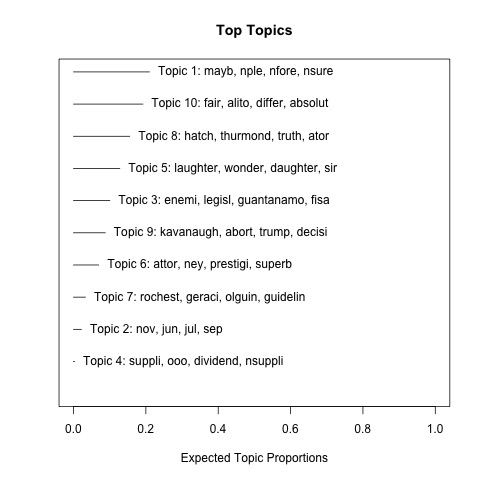
\includegraphics[height = 175mm, width = 175mm]{../tables_figures/stm_male_frex.jpg}
    \caption{Predicted proportion of topics with 5 top words based on their FREX.}
    \label{fig:frex_male}
\end{figure}
	    
Figures \ref{fig:frex_poc} and \ref{fig:frex_male} tell us little substantively about the topics. We obtain the 5 words in each topic with the highest FREX. FREX represents words that are both exclusive to and frequent in that particular topic.

Looking first at \ref{fig:frex_poc} we see that topic 1 for example includes words that can be thought of to represent the topic well seem to discuss the nominee's personal life such as lemmatized words getting at religion, their hobbies, what car they own. Looking at a topic associated with white nominees such as 5, we also see that the topic seems to discuss the nominee's leisure activities but paint a picture of an intellectual nominee who spends time reading. Of the other topics highlighted for their association with nominees of color and comparing that to topics associated with white nominees, seem to show substantive differences that fit with what we might expect if we see racial bias. Particularly that topics associated with white nominees seem to include a lot of lemmatized words depicting a more academic nominee.

Next, looking at \ref{fig:frex_male} we also observe a number of interesting FREX words in topics associated to represent topics often associated with female nominees compared to the FREX words in topics associated to represent topics covered for male nominees. For example, topic 7 was identified for its association with female nominees. In topic 7, we see FREX words such as correct and remember. Topic 22, also includes words associated with statement qualifiers such as ``think". Topic 12 which is positively associated with male nominees include words such as ``argument" and ``decide" instead.

We admit that there is a lot of interpretation in what these FREX words mean and how they might present bias. However, they do show some interesting differences when we consider the operational purpose of these words in common usage - as we highlight in our discussion of Figures \ref{fig:stm_poc} and \ref{fig:stm_male}. Further, some of the FREX words included depict topics that are not entirely clear what pattern it is supposed to represent - again concern with choosing more than 30 topics was parsimony. Thankfully, overall, we do see most of our topics, as represented by the 5 lemmatized words with the highest FREX, have some clarity about what to take away from it.

	    
\section{Conclusions}

As the public are not immune to relying on gender and racial biases to criticize policy and candidates who are associated with a particular racial or gender category, differences in how members of congress evaluate nominees for federal positions are likely to also contain similar racial and gender biases; particularly when it is a candidate holding a different ideological position as a given committee member. As nominees for federal offices are caught up in the increasingly polarized congress, challenges on their qualifications are likely to become more prevalent. As ideological differences are not effective arguments for questioning one's qualifications - well, at least for the most part - committee members may rely on their racial and gender biases to bring up concerns about a nominee's qualifications. 

In this paper, we predicted that there would be gendered-and-racially-based differences in how Federal Judiciary nominees were treated in their confirmation hearings. First, we tested whether female or nominees of color were interrupted more during their hearings relative to their male and white colleagues. The interruptions hypothesis had no support. Second, we tested whether female or nominees of color had different topics discussed during their hearings than their male or white counterparts. Analyses demonstrate that there are some substantive differences in topics and that they follow what one might expect given commonly-held racial and gendered stereotypes in politics. 

Intersectionality is excluded from this analysis, but is shown to have very important effects on political events \citep[see][]{phillips_2020_oxford}. That is, not all women and not all people of a particular racial category have the same experiences. Black women have different experiences than Black men. White women have very different experiences than Latinas. Further work should explicitly consider the role of intersectionality.

Further work should also take up the task of exploring the heterogeneity in experiences of nomination for federal office outside of the court. While there is an air of separation from politics in the court, nominees for bureaucratic offices and cabinet positions may see more heterogeneity in experiences in partisanship - and it may dominate explanations for that heterogeneity. However, this is an open area. With advances in text analysis methods and improvements in computational capabilities for the average researcher, there are a number of opportunities to take advantage of published transcripts from committee hearings, not just for confirmation hearings for nominees of the court. 


\newpage
\bibliographystyle{apsr}
\bibliography{../Literature/tpg_dcr_judicial_interruptions.bib}

\end{document}
